\documentclass[a4paper,11pt]{article}
\usepackage{xcolor}
\usepackage{tikz}
%\usepackage{tkz-euclide}
\usetikzlibrary{shapes.geometric, arrows.meta}
 \tikzstyle{startstop} = [rectangle, rounded corners, minimum width=3cm, minimum height=1cm,text centered, draw=black]
\tikzstyle{process} = [rectangle, minimum width=3cm, minimum height=1cm, text centered, text width=3cm, draw=black]
\tikzstyle{decision} = [diamond, minimum width=4cm,  minimum height=2cm, text centered, draw=black, aspect=2, inner sep=-1ex]
\tikzstyle{arrow} = [thick,->,>=Latex]
\begin{document}
\begin{figure}[h!]
\begin{center}
 \scalebox{0.85}{
 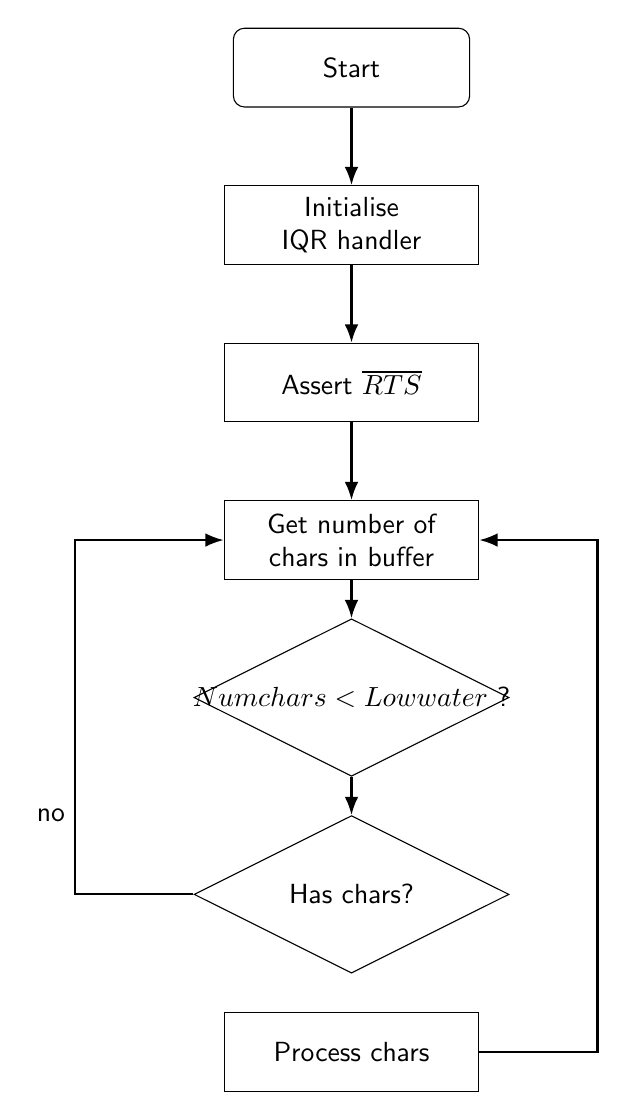
\begin{tikzpicture}[font=\sffamily,node distance=2cm]
 	\node (start) [startstop] {Start};
 	\node (init) [process, below of=start] {Initialise IQR handler};
 	\node (assertrts) [process, below of=init] {Assert $\overline{RTS}$};
 	\node (checkbuf) [process, below of=assertrts] {Get number of chars in buffer};
 	\node (minlevel) [decision, below of=checkbuf] {$Num chars <
 		   Low water$ ?};
 	\node (haschars) [decision, below of=minlevel, yshift=-0.5cm] {Has chars?};
 	\node (procchars) [process, below of=haschars] {Process chars};

%	\node (start) [startstop] {Receive Routine};
%	\node (status) [process, below of=start] {Read Status};
%	\node (rdre) [decision, below of=status, yshift=-1cm] {Is $RDRE$ = 1 ?};
%	\node (load) [process, below of=tdre, yshift=-1cm] {Load Character};
%	\node (rts) [startstop, below of=load] {Return};
%	\node (cts) [decision, right of=tdre, xshift=3.5cm] {Is $\overline{CTS}$ = 0 ?};
%	\node (error) [process, below of=cts, yshift=-1cm] {Loss of Carrier Error Routine};

	\draw [arrow] (start) -- (init);
	\draw [arrow] (init) -- (assertrts);
	\draw [arrow] (assertrts) -- (checkbuf);
	\draw [arrow] (checkbuf) -- (minlevel);
	\draw [arrow] (minlevel) -- (haschars);
	\draw [arrow] (haschars.west) -| ++(-1.5cm,1cm) node[anchor=east] {no} |- (checkbuf.west);
	\draw [arrow] (procchars.east) -| ++(1.5cm,1cm) node {} |- (checkbuf.east);

%	\draw [arrow] (haschars) -| node[anchor=north west] {no} (checkbuf);
%	\draw [arrow] (load) -- (rts);
%	\draw [arrow] (tdre) -- node[anchor=south] {no} (cts);
%	\draw [arrow] (cts) |- node[anchor=north west] {no} (status);
%	\draw [arrow] (cts) -- node[anchor=west] {yes} (error);
 \end{tikzpicture}
 }
 \caption{Receive subroutine.}
 \label{fig:flowctl}
\end{center}
\end{figure}
\end{document}



